% This file was created with tikzplotlib v0.10.1.
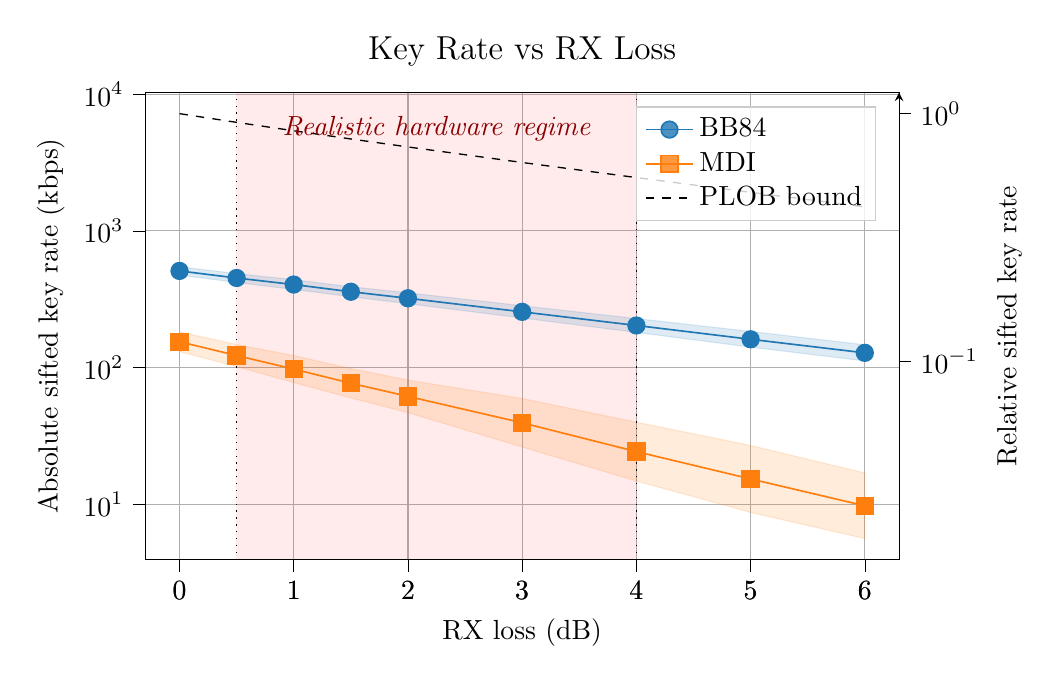
\begin{tikzpicture}
\definecolor{darkgray176}{RGB}{176,176,176}
\definecolor{darkorange25512714}{RGB}{255,127,14}
\definecolor{darkred}{RGB}{139,0,0}
\definecolor{dimgray}{RGB}{105,105,105}
\definecolor{lightgray204}{RGB}{204,204,204}
\definecolor{steelblue31119180}{RGB}{31,119,180}
\begin{axis}[
width=0.92\linewidth,
height=0.62\linewidth,
legend cell align={left},
legend pos=north east,
legend style={fill opacity=0.8, draw opacity=1, text opacity=1, draw=lightgray204, font=\fontsize{10}{12}\selectfont},
log basis y={10},
tick align=outside,
tick pos=left,
tick label style={font=\fontsize{10}{12}\selectfont},
label style={font=\fontsize{10}{12}\selectfont},
title style={font=\fontsize{12}{14}\selectfont},
x grid style={darkgray176},
xlabel={RX loss (dB)},
xmajorgrids,
xmin=-0.3, xmax=6.3,
xtick style={color=black},
xtick={-1,0,1,2,3,4,5,6,7},
xticklabels={
  \(\displaystyle {\ensuremath{-}1}\),
  \(\displaystyle {0}\),
  \(\displaystyle {1}\),
  \(\displaystyle {2}\),
  \(\displaystyle {3}\),
  \(\displaystyle {4}\),
  \(\displaystyle {5}\),
  \(\displaystyle {6}\),
  \(\displaystyle {7}\)
},
y grid style={darkgray176},
ylabel={Absolute sifted key rate (kbps)},
ymajorgrids,
ymin=3.92960955757881, ymax=10295.6818836118,
ymode=log,
ytick style={color=black},
ytick={0.1,1,10,100,1000,10000,100000,1000000},
yticklabels={
  \(\displaystyle {10^{-1}}\),
  \(\displaystyle {10^{0}}\),
  \(\displaystyle {10^{1}}\),
  \(\displaystyle {10^{2}}\),
  \(\displaystyle {10^{3}}\),
  \(\displaystyle {10^{4}}\),
  \(\displaystyle {10^{5}}\),
  \(\displaystyle {10^{6}}\)
}
]
\path [draw=red, fill=red, opacity=0.08]
(axis cs:0.5,3.92960955757881)
--(axis cs:0.5,10295.6818836118)
--(axis cs:4,10295.6818836118)
--(axis cs:4,3.92960955757881)
--cycle;
\path [draw=steelblue31119180, fill=steelblue31119180, opacity=0.15]
(axis cs:0,545.940392593672)
--(axis cs:0,475.296195264291)
--(axis cs:0.5,419.771403108569)
--(axis cs:1,373.347955397291)
--(axis cs:1.5,329.982293929978)
--(axis cs:2,293.382221566412)
--(axis cs:3,230.57627059771)
--(axis cs:4,181.090003579346)
--(axis cs:5,141.196476546638)
--(axis cs:6,111.981870705518)
--(axis cs:6,146.849311065689)
--(axis cs:6,146.849311065689)
--(axis cs:5,183.89904107419)
--(axis cs:4,228.268358056456)
--(axis cs:3,283.678366576257)
--(axis cs:2,352.250914982713)
--(axis cs:1.5,390.245951517817)
--(axis cs:1,439.399348895853)
--(axis cs:0.5,486.985550719261)
--(axis cs:0,545.940392593672)
--cycle;
\path [draw=darkorange25512714, fill=darkorange25512714, opacity=0.15]
(axis cs:0,182.445540778052)
--(axis cs:0,131.08894894332)
--(axis cs:0.5,101.805769865286)
--(axis cs:1,77.759570111513)
--(axis cs:1.5,60.0246045303552)
--(axis cs:2,46.858665266394)
--(axis cs:3,26.2402369905027)
--(axis cs:4,14.8128600873516)
--(axis cs:5,8.73320643083954)
--(axis cs:6,5.61987859707551)
--(axis cs:6,16.9641891633235)
--(axis cs:6,16.9641891633235)
--(axis cs:5,26.944340758267)
--(axis cs:4,39.8939023597603)
--(axis cs:3,59.4619037237268)
--(axis cs:2,81.0230475659468)
--(axis cs:1.5,98.4827615764615)
--(axis cs:1,122.400039308043)
--(axis cs:0.5,147.601290965608)
--(axis cs:0,182.445540778052)
--cycle;
\addplot [semithick, steelblue31119180, mark=*, mark size=3, mark options={solid}]
table {%
0 509.39512310275
0.5 452.131184413355
1 405.02944153872
1.5 358.851298282082
2 321.471858778385
3 255.752809983397
4 203.315316140952
5 161.139370235772
6 128.235956599357
};
\addlegendentry{BB84}
\addplot [semithick, darkorange25512714, mark=square*, mark size=3, mark options={solid}]
table {%
0 154.649908438352
0.5 122.583290296287
1 97.5590817824035
1.5 76.8855566194611
2 61.6168147891128
3 39.5005625987408
4 24.3093149634784
5 15.339833440583
6 9.76405057318438
};
\addlegendentry{MDI}
\addplot [line width=0.48pt, black, dotted, forget plot]
table {%
0.5 3.92960955757881
0.5 10295.6818836118
};
\addplot [line width=0.48pt, black, dotted, forget plot]
table {%
4 3.92960955757881
4 10295.6818836118
};
\addplot [line width=0.48pt, black, dashed]
table {%
0 7199.08966586673
0.5 6218.00544236189
1 5396.51990139278
1.5 4701.82229005165
2 4109.66352927759
3 3163.45843492322
4 2453.7254764658
5 1913.83615732177
6 1498.93553119322
};
\addlegendentry{PLOB bound}
\draw (axis cs:0.4208,0.01) node[
  font=\fontsize{10}{12}\selectfont,
  anchor=south east,
  text=dimgray,
  rotate=0.0
]{0.5};
\draw (axis cs:2.25,8130.288260537779) node[
  font=\fontsize{10}{12}\selectfont,
  anchor=north,
  text=darkred,
  rotate=0.0
]{\itshape Realistic hardware regime};
\end{axis}
\begin{axis}[
width=0.92\linewidth,
height=0.62\linewidth,
axis y line=right,
log basis y={10},
tick align=outside,
tick label style={font=\fontsize{10}{12}\selectfont},
label style={font=\fontsize{10}{12}\selectfont},
title style={font=\fontsize{12}{14}\selectfont},
title={Key Rate vs RX Loss},
x grid style={darkgray176},
xmin=-0.3, xmax=6.3,
xtick pos=left,
xtick style={color=black},
y grid style={darkgray176},
ylabel={Relative sifted key rate},
ymin=0.0157291045553096, ymax=1.21862824016205,
ymode=log,
ytick pos=right,
ytick style={color=black},
ytick={0.001,0.01,0.1,1,10,100},
yticklabel style={anchor=west},
yticklabels={
  \(\displaystyle {10^{-3}}\),
  \(\displaystyle {10^{-2}}\),
  \(\displaystyle {10^{-1}}\),
  \(\displaystyle {10^{0}}\),
  \(\displaystyle {10^{1}}\),
  \(\displaystyle {10^{2}}\)
}
]
\addplot [semithick, steelblue31119180, opacity=0, mark=*, mark size=3, mark options={solid}]
table {%
0 1
0.5 0.887584438695453
1 0.795118412346916
1.5 0.704465516073853
2 0.631085466268866
3 0.502071571525055
4 0.399130865059227
5 0.31633473295595
6 0.251741626064785
};
\addplot [semithick, darkorange25512714, opacity=0, mark=square*, mark size=3, mark options={solid}]
table {%
0 0.303595188537283
0.5 0.240644805450093
1 0.191519465652059
1.5 0.150935007290897
2 0.120960747354238
3 0.0775440533433871
4 0.0477219232398796
5 0.0301138207746226
6 0.0191679310035618
};
\end{axis}
\end{tikzpicture}
